\documentclass[11pt]{article}

% ============================================================
%  Beyond curl-noise: helicity and phase coherence controls
%  for divergence-free flow fields
%  Standalone preprint. Compile: pdflatex main; pdflatex main
% ============================================================

\usepackage[margin=1in]{geometry}
\usepackage{amsmath,amssymb,amsthm}
\usepackage{mathtools}
\usepackage{booktabs}
\usepackage{graphicx}
\usepackage{microtype}
\usepackage[table]{xcolor}
\usepackage{enumitem}
\usepackage[hidelinks]{hyperref}
\graphicspath{{figures/}}

% Float placement: keep figures near their first reference (they were all
% deferred to the end otherwise). Relax the default fraction limits so more of
% a page may be occupied by floats, and allow more top/bottom floats per page.
\usepackage{placeins}   % \FloatBarrier to pin figures within their section
\renewcommand{\topfraction}{0.9}
\renewcommand{\bottomfraction}{0.9}
\renewcommand{\textfraction}{0.08}
\renewcommand{\floatpagefraction}{0.7}
\setcounter{topnumber}{3}
\setcounter{bottomnumber}{2}
\setcounter{totalnumber}{4}

\newtheorem{proposition}{Proposition}
\newtheorem{lemma}{Lemma}
\theoremstyle{remark}
\newtheorem{remark}{Remark}

\newcommand{\R}{\mathbb{R}}
\newcommand{\Z}{\mathbb{Z}}
\newcommand{\C}{\mathbb{C}}
\newcommand{\bx}{\mathbf{x}}
\newcommand{\bk}{\mathbf{k}}
\newcommand{\bu}{\mathbf{u}}
\newcommand{\bA}{\mathbf{A}}
\newcommand{\bn}{\mathbf{n}}
\newcommand{\bomega}{\boldsymbol{\omega}}
\newcommand{\he}{\mathbf{h}}
\newcommand{\khat}{\hat{\bk}}
\newcommand{\ehat}{\hat{\mathbf{e}}}
\DeclareMathOperator{\curl}{curl}
\DeclareMathOperator{\dvg}{div}

\title{\bfseries Beyond curl-noise: helicity and phase coherence controls\\
for divergence-free flow fields}
\author{Rifat Jumagulov\\
\small \texttt{jum.rifm@gmail.com}}
\date{July 11, 2026}

\begin{document}
\maketitle

\begin{figure}[htbp]
  \centering
  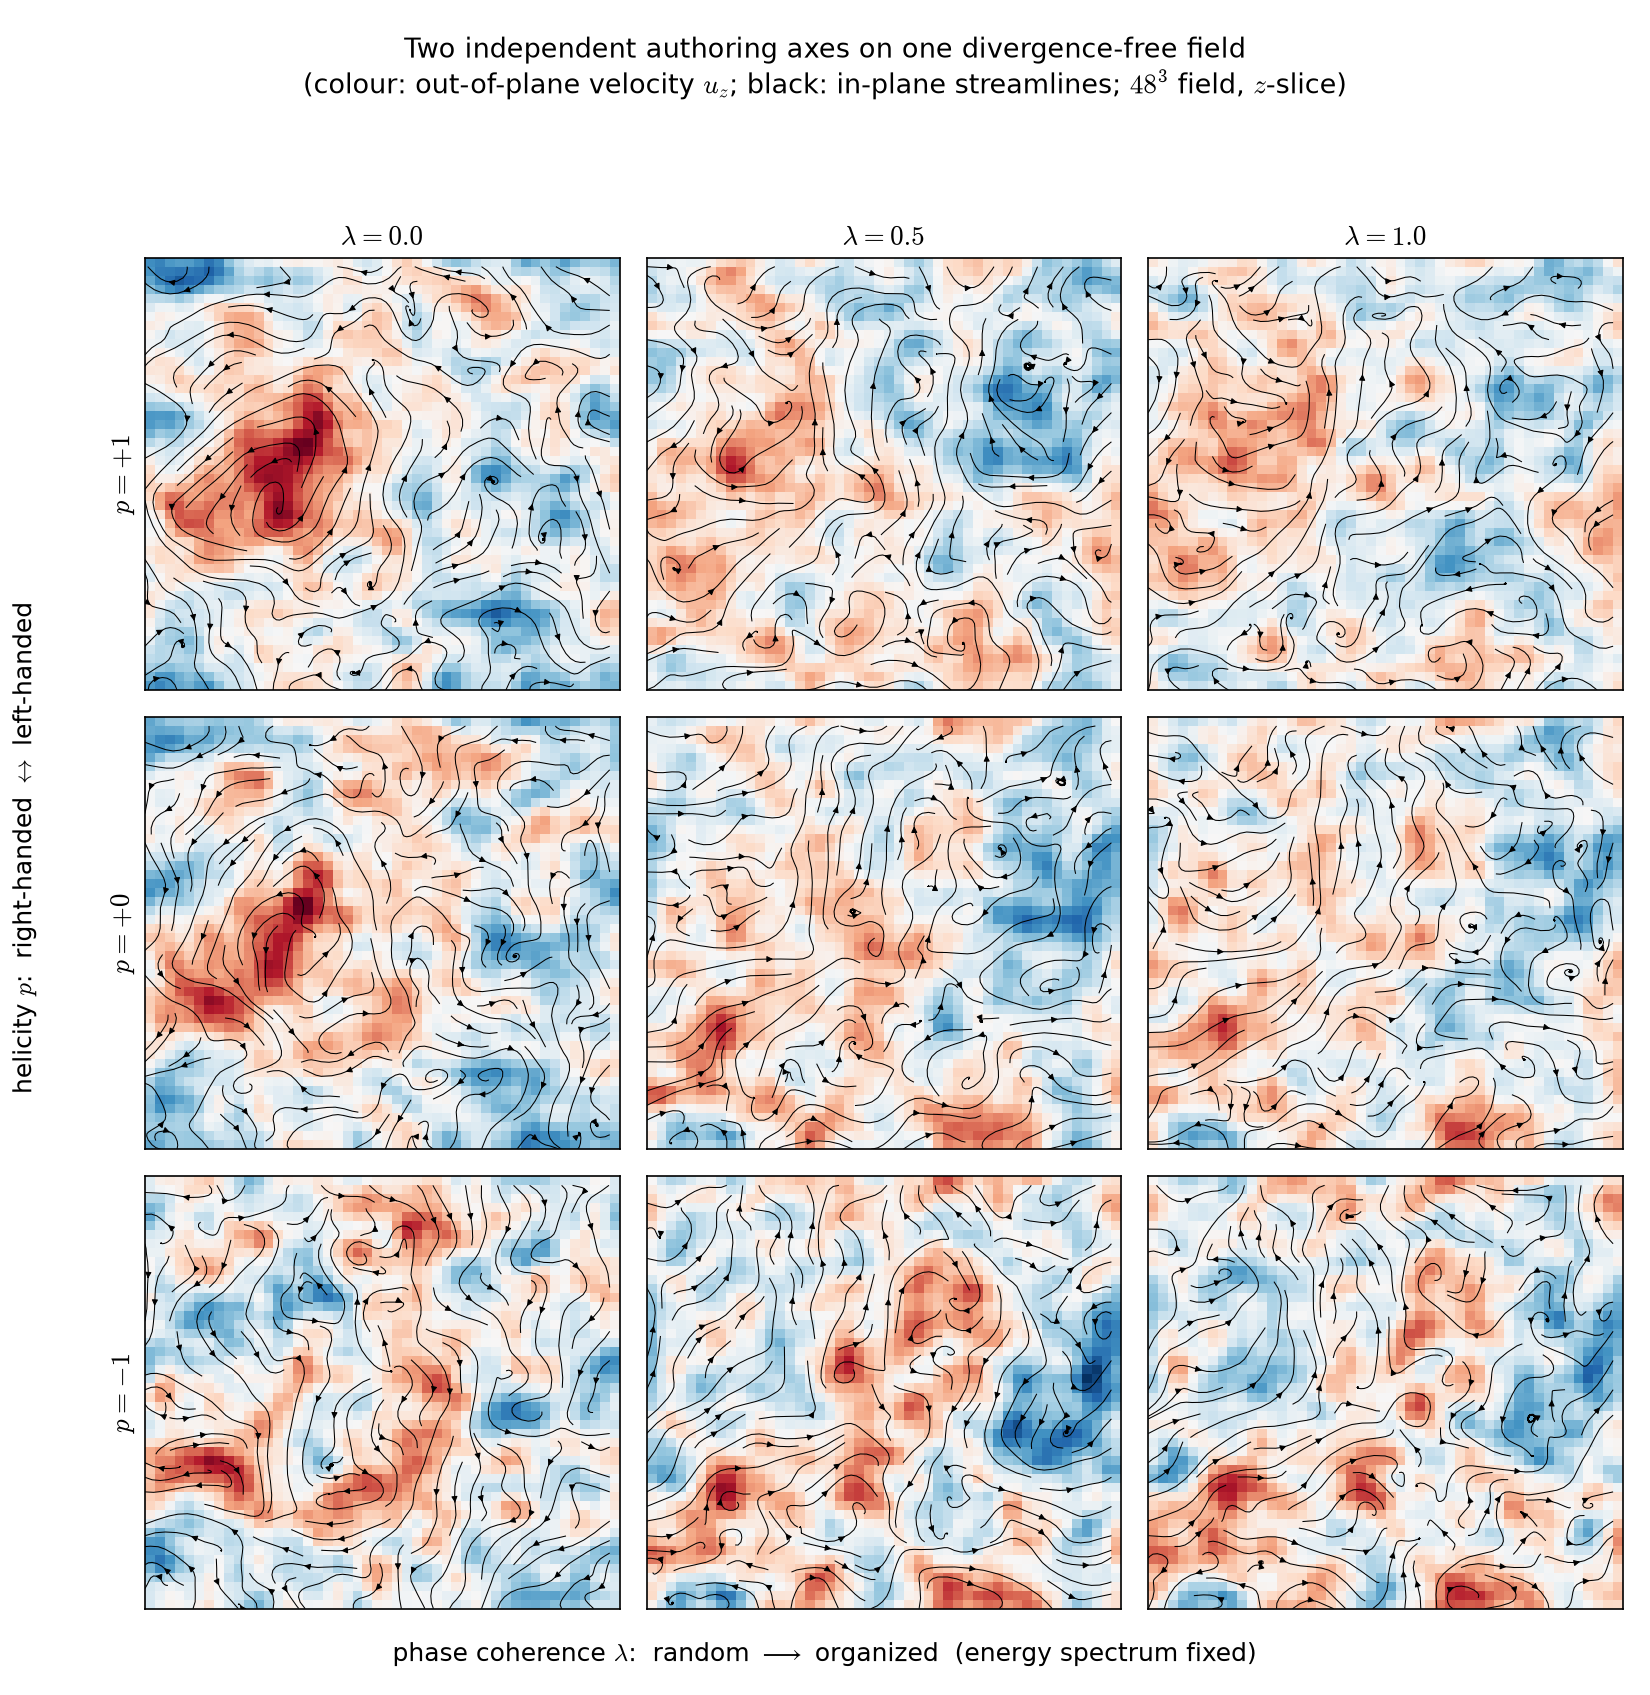
\includegraphics[width=0.86\linewidth]{figures/gallery.png}
  \caption{Two independent authoring axes on a single divergence-free field.
    \textbf{Left to right:} the phase-coherence knob $\lambda$ (\S\ref{sec:coherence})
    carries the field from random-phase noise to organized structure \emph{at a fixed
    power spectrum} (the vortices sharpen and separate as you move right). \textbf{Top to
    bottom:} the helicity knob $p$ (\S\ref{sec:helicity}) sweeps the chirality from
    right- to left-handed---read it in the colour, which is the out-of-plane velocity:
    the top row leans one sign (its swirls corkscrew out of the page), the middle row is
    balanced (mixed colour, no preferred twist), and the bottom row leans the opposite
    sign (swirls corkscrew into the page). The layout of the streamlines is otherwise the
    same down each column; only the handedness flips. The two are orthogonal: across
    every row the total energy is identical to four significant figures, and the net
    helicity $\int\bu\cdot\bomega$ is set by $p$ alone ($+6.3\cdot10^{-4}$, $0$,
    $-6.4\cdot10^{-4}$ for the three rows) and is unchanged by $\lambda$ to machine
    precision. Colour is the out-of-plane velocity $u_z$; black curves are in-plane
    streamlines; each panel is a $z$-slice of a $48^3$ field.}
  \label{fig:teaser}
\end{figure}

\begin{abstract}
We present a solver-free method for synthesizing divergence-free vector fields for the
procedural animation of smoke, particles, and other advected media, giving the artist three
independent dials on top of the usual noise: the spectral slope (how ragged versus silky the
flow looks), the \emph{helicity} (whether the swirls corkscrew left or right), and the
\emph{phase coherence} (whether the motion organizes into distinct rolling vortices or stays
an even haze). The construction works in the frequency domain on the \emph{helical} basis---the
natural directions in which a swirl reinforces its own rotation---which is divergence-free by
construction and turns handedness into a single dial, continuous from mirror-symmetric (no
preferred twist) to maximally helical (every swirl fully corkscrewed, a Beltrami field). The
phase-coherence dial is, to our knowledge, new to procedural flow: it slides the field from
formless noise to organized filaments while holding the amount of motion at every scale fixed,
so the flow reorganizes without speeding up or slowing down---an axis that curl-noise does not
expose. We show that making the field real-valued (the step every graphics implementation
needs) does not wash out the chosen handedness, give the construction in two and three
dimensions, and provide two interchangeable ways to evaluate it: an FFT bake for offline
authoring and an analytic mode-sum that runs per pixel in a fragment shader (GLSL included).
Solid obstacles are handled in the same framework by ramping the vector potential before the
curl, which keeps the field exactly divergence-free and tangent to the surface with no solver
and no pressure projection. The payoff for the artist is direct control over how a flow twists
and how tightly it organizes---qualities that ordinary curl-noise leaves fixed---at no run-time
cost downstream.
\end{abstract}

\section{Introduction}

Procedural flow fields are a workhorse of visual effects: rather than simulate a fluid, one
generates a static or slowly-evolving velocity field and advects particles, smoke density,
or other tracers through it. The field must be \emph{divergence-free} so that tracers are
transported without spurious compression or rarefaction. The standard construction is
\emph{curl-noise}~\cite{bridson2007}: take a vector (or scalar) noise
potential~\cite{perlin1985} and use its curl, which is divergence-free identically. Curl-noise
is cheap, tileable with care, and ubiquitous, and it sits within a broad family of procedural
noise functions~\cite{lagae2010}, some of which already expose spectral control by
example~\cite{galerne2012}. It has itself been extended in recent years---boundary-respecting
pointwise variants~\cite{chang2022} and differentiable formulations~\cite{ding2023}---but these
enlarge its geometry and controllability rather than the two qualities we target below.

Its expressive range is, however, narrow. Curl-noise is isotropic and exposes essentially two
knobs---frequency and amplitude. This paper adds three dials to a divergence-free field. One,
the spectral slope, sharpens control the broader noise family already offers in weaker
forms~\cite{lagae2010,galerne2012} into an exact per-scale envelope (\S\ref{sec:construction}).
The other two are qualities that distinguish real turbulent flow and that no curl-noise variant
exposes directly:
\begin{itemize}[nosep]
\item \textbf{Helicity} (chirality): whether the swirls of the flow corkscrew left or right.
Watch a dye streak carried by the field---a right-handed flow winds it into a clockwise helix,
a left-handed one into its mirror, and a mirror-symmetric flow shows no preference.
Quantitatively, helicity $\int \bu\cdot\bomega\,d\bx$ is a genuine three-dimensional invariant
of ideal flow~\cite{moffatt1969}; a field can range from mirror-symmetric to fully helical
(a Beltrami field, $\bomega\parallel\bu$, in which every swirl is maximally
corkscrewed)~\cite{constantin1988,dombre1986}.
\item \textbf{Phase organization}: whether the motion lines up into distinct rolling vortices
or stays an even, structureless haze. At a \emph{fixed} power spectrum---the same amount of
motion at every scale, so the flow neither speeds up nor slows down---a field with random
inter-mode phases looks featureless (Gaussian), whereas correlated phases pull that same energy
into coherent filaments and sheets. That the phases, not the amplitude spectrum, carry the
structural information of a field is well established in turbulence and in
cosmology~\cite{coles2000}.
\end{itemize}

We build the field directly in the frequency domain from a prescribed spectral tensor, which
makes both qualities into explicit controls while retaining exact divergence-freeness
(Fig.~\ref{fig:teaser}). The contributions are:
\begin{enumerate}[nosep]
\item a divergence-free spectral construction with a single \emph{helicity} parameter
$p\in[-1,1]$, realized on the helical basis of Waleffe and of Craya--Herring
(\S\ref{sec:helical}), and reducing in two dimensions to a stream-function curl
(\S\ref{sec:construction});
\item a proof that the Hermitian symmetrization required to obtain a \emph{real} field
preserves the helicity polarization---the bias is not washed out by making the field real
(\S\ref{sec:hermitian}, Proposition~\ref{prop:pres});
\item a \emph{phase-coherence} control that interpolates inter-mode phases from random to
structured at fixed power spectrum (\S\ref{sec:coherence});
\item an analytic Beltrami mode-sum variant that evaluates per pixel with no FFT, suitable
for a real-time fragment shader, together with its exact and statistical properties
(\S\ref{sec:modesum});
\item a solid-obstacle treatment that ramps the vector potential before taking the curl,
keeping the field exactly divergence-free and tangent to the surface---free-slip and
no-penetration---for any obstacle shape, with no solver (\S\ref{sec:obstacles});
\item numerical validation of divergence-freeness, reality, helicity control, and the
obstacle guarantees for both constructions (\S\ref{sec:validation}, \S\ref{sec:obstacles}).
\end{enumerate}
The method is an authoring/bake tool in the spirit of spectral turbulence synthesis for
graphics~\cite{stam1993,kim2008}; \S\ref{sec:discussion} positions it against curl-noise and
states its limits.

\FloatBarrier
\section{Divergence-free spectral fields}
\label{sec:construction}

We work on a periodic box $\mathbb{T}^d=[0,2\pi)^d$, $d\in\{2,3\}$, with wavevectors
$\bk\in\Z^d$. A field
$\bu(\bx)=\sum_{\bk}\hat\bu(\bk)\,e^{i\bk\cdot\bx}$
is divergence-free iff $\bk\cdot\hat\bu(\bk)=0$ for every $\bk$. The spectral slope enters
through a radial envelope
\begin{equation}
E(\bk) = |\bk|^{-s}\,e^{-|\bk|^2/k_c^2},
\label{eq:env}
\end{equation}
with slope $s$ and a smooth high-frequency cutoff $k_c$. Steep $s$ concentrates energy in a
few large scales (smooth, silky flow); shallow $s$ spreads it across scales (fine, ragged
flow) (Fig.~\ref{fig:slope}).

\begin{figure}[htbp]
  \centering
  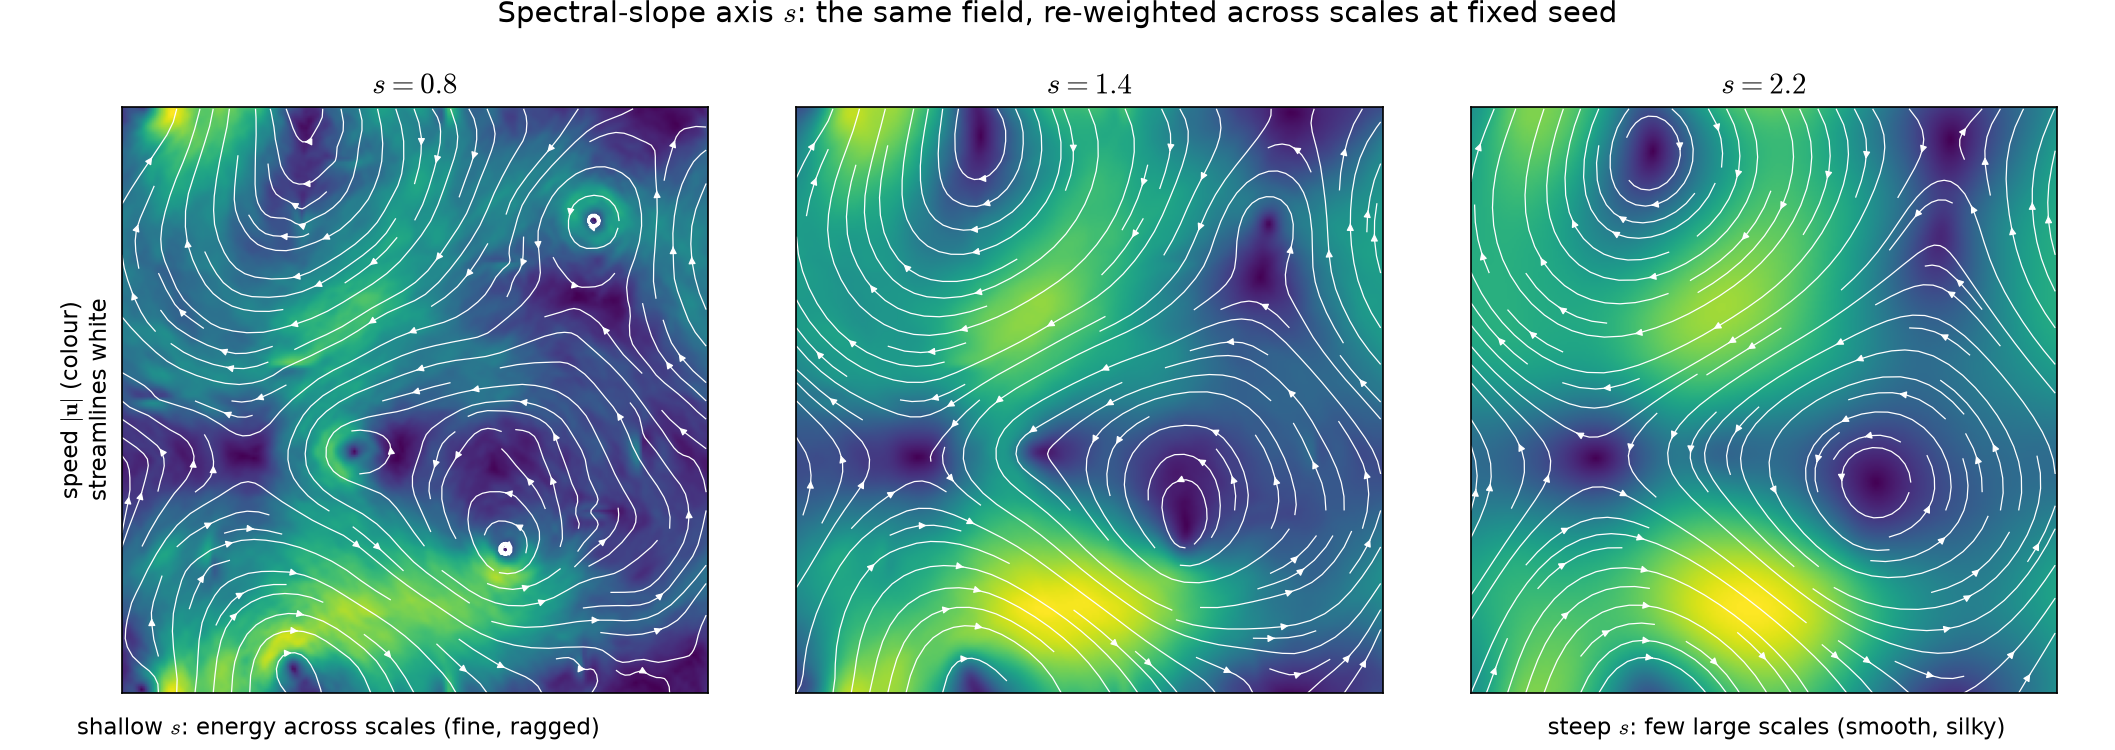
\includegraphics[width=\linewidth]{figures/slope.png}
  \caption{The spectral-slope axis $s$ of the envelope~\eqref{eq:env}, on one
    two-dimensional field at fixed random seed and phase coherence. Colour is
    speed $|\bu|$, white curves are streamlines. A shallow slope spreads
    energy across scales (fine, ragged flow); a steep slope concentrates it in a
    few large scales (smooth, silky flow). Slope re-weights the \emph{same} modes,
    so the large-scale skeleton persists while fine detail is added or removed.}
  \label{fig:slope}
\end{figure}

\subsection{Two dimensions: curl of a stream function}
In two dimensions every divergence-free field is the curl of a scalar stream function
$\psi$, $\bu=(\partial_y\psi,-\partial_x\psi)$. Prescribing a vorticity spectrum
$\hat\omega(\bk)$ and setting $\hat\psi=\hat\omega/|\bk|^2$ gives
\begin{equation}
\hat u(\bk) = -\,i\,\frac{k_y}{|\bk|^2}\,\hat\omega(\bk), \qquad
\hat v(\bk) = +\,i\,\frac{k_x}{|\bk|^2}\,\hat\omega(\bk),
\label{eq:2d}
\end{equation}
which satisfies $\bk\cdot\hat\bu(\bk)=0$ identically. There is no helicity in two dimensions;
the only chirality available is the \emph{sign} of the scalar vorticity, which biases whether
vortices turn clockwise or counter-clockwise. We treat the genuine helicity control in three
dimensions.

\subsection{Three dimensions: the helical basis}
\label{sec:helical}
The idea in one sentence: instead of describing each wave by its $x$-, $y$-, $z$-components,
we describe it by how much it corkscrews clockwise versus counter-clockwise. These two
corkscrew directions are the \emph{helical} vectors below. They are special because the curl
operator---the thing that measures local rotation---simply scales them rather than mixing them
(they are its eigenvectors, \eqref{eq:eigen}), so a swirl built from one of them reinforces its
own rotation. Working in this basis makes handedness a single number and keeps the field
divergence-free automatically.

For each $\bk\ne\mathbf 0$ choose a real orthonormal transverse frame
$(\ehat_1,\ehat_2)$ with $\ehat_1,\ehat_2\perp\bk$ and $\{\ehat_1,\ehat_2,\khat\}$
right-handed ($\khat=\bk/|\bk|$). This is the Craya--Herring frame~\cite{herring1974}. Define
the two \emph{helical} vectors~\cite{waleffe1992,constantin1988}
\begin{equation}
\he_\pm(\bk) = \frac{\ehat_1 \pm i\,\ehat_2}{\sqrt 2}.
\label{eq:helical}
\end{equation}
They are transverse and are the eigenvectors of the curl operator in Fourier space:
\begin{equation}
\he_\pm\cdot\bk = 0,
\qquad
i\,\bk\times\he_\pm = \pm\,|\bk|\,\he_\pm .
\label{eq:eigen}
\end{equation}
Any divergence-free field expands as
$\hat\bu(\bk)=a_+(\bk)\he_+(\bk)+a_-(\bk)\he_-(\bk)$, and the construction assigns the
amplitudes $a_\pm$ their envelope and phase (\S\ref{sec:helicity}--\S\ref{sec:coherence}).
Transversality of $\he_\pm$ guarantees $\dvg\bu\equiv 0$ regardless of the amplitudes.

\FloatBarrier
\section{Helicity as a polarization control}
\label{sec:helicity}

In plain terms, this section builds the left/right corkscrew dial. Because the helical basis
already separates clockwise swirls from counter-clockwise ones, biasing the handedness is just
a matter of putting more energy into one than the other: a single number $p\in[-1,1]$ slides
from all-left through balanced to all-right. Everything below makes that precise.

The helicity of the field is diagonal in the helical basis. Writing
$\bomega=\curl\bu$ and using~\eqref{eq:eigen},
\begin{equation}
\mathcal H \;=\; \int_{\mathbb T^3} \bu\cdot\bomega\,d\bx
\;=\; \sum_{\bk} |\bk|\big(\,|a_+(\bk)|^2 - |a_-(\bk)|^2\,\big).
\label{eq:helicity}
\end{equation}
We therefore split each mode's energy between the two channels by a single
\emph{helicity parameter} $p\in[-1,1]$:
\begin{equation}
|a_+(\bk)|^2 = \tfrac{1+p}{2}\,E(\bk)^2, \qquad
|a_-(\bk)|^2 = \tfrac{1-p}{2}\,E(\bk)^2,
\label{eq:split}
\end{equation}
so that $p$ biases $\mathcal H$ directly. At $p=0$ the two channels carry equal energy and
the field is statistically mirror-symmetric ($\mathcal H=0$ in the mean). At $p=\pm1$ all
energy is in one channel and the field is a pure helical (Beltrami) field,
$\bomega=\pm|\bk|\,\bu$ mode-by-mode, i.e.\ $\bomega\parallel\bu$; the ABC
flows~\cite{dombre1986} are the classical single-mode example
(Fig.~\ref{fig:helix}).

\begin{figure}[htbp]
  \centering
  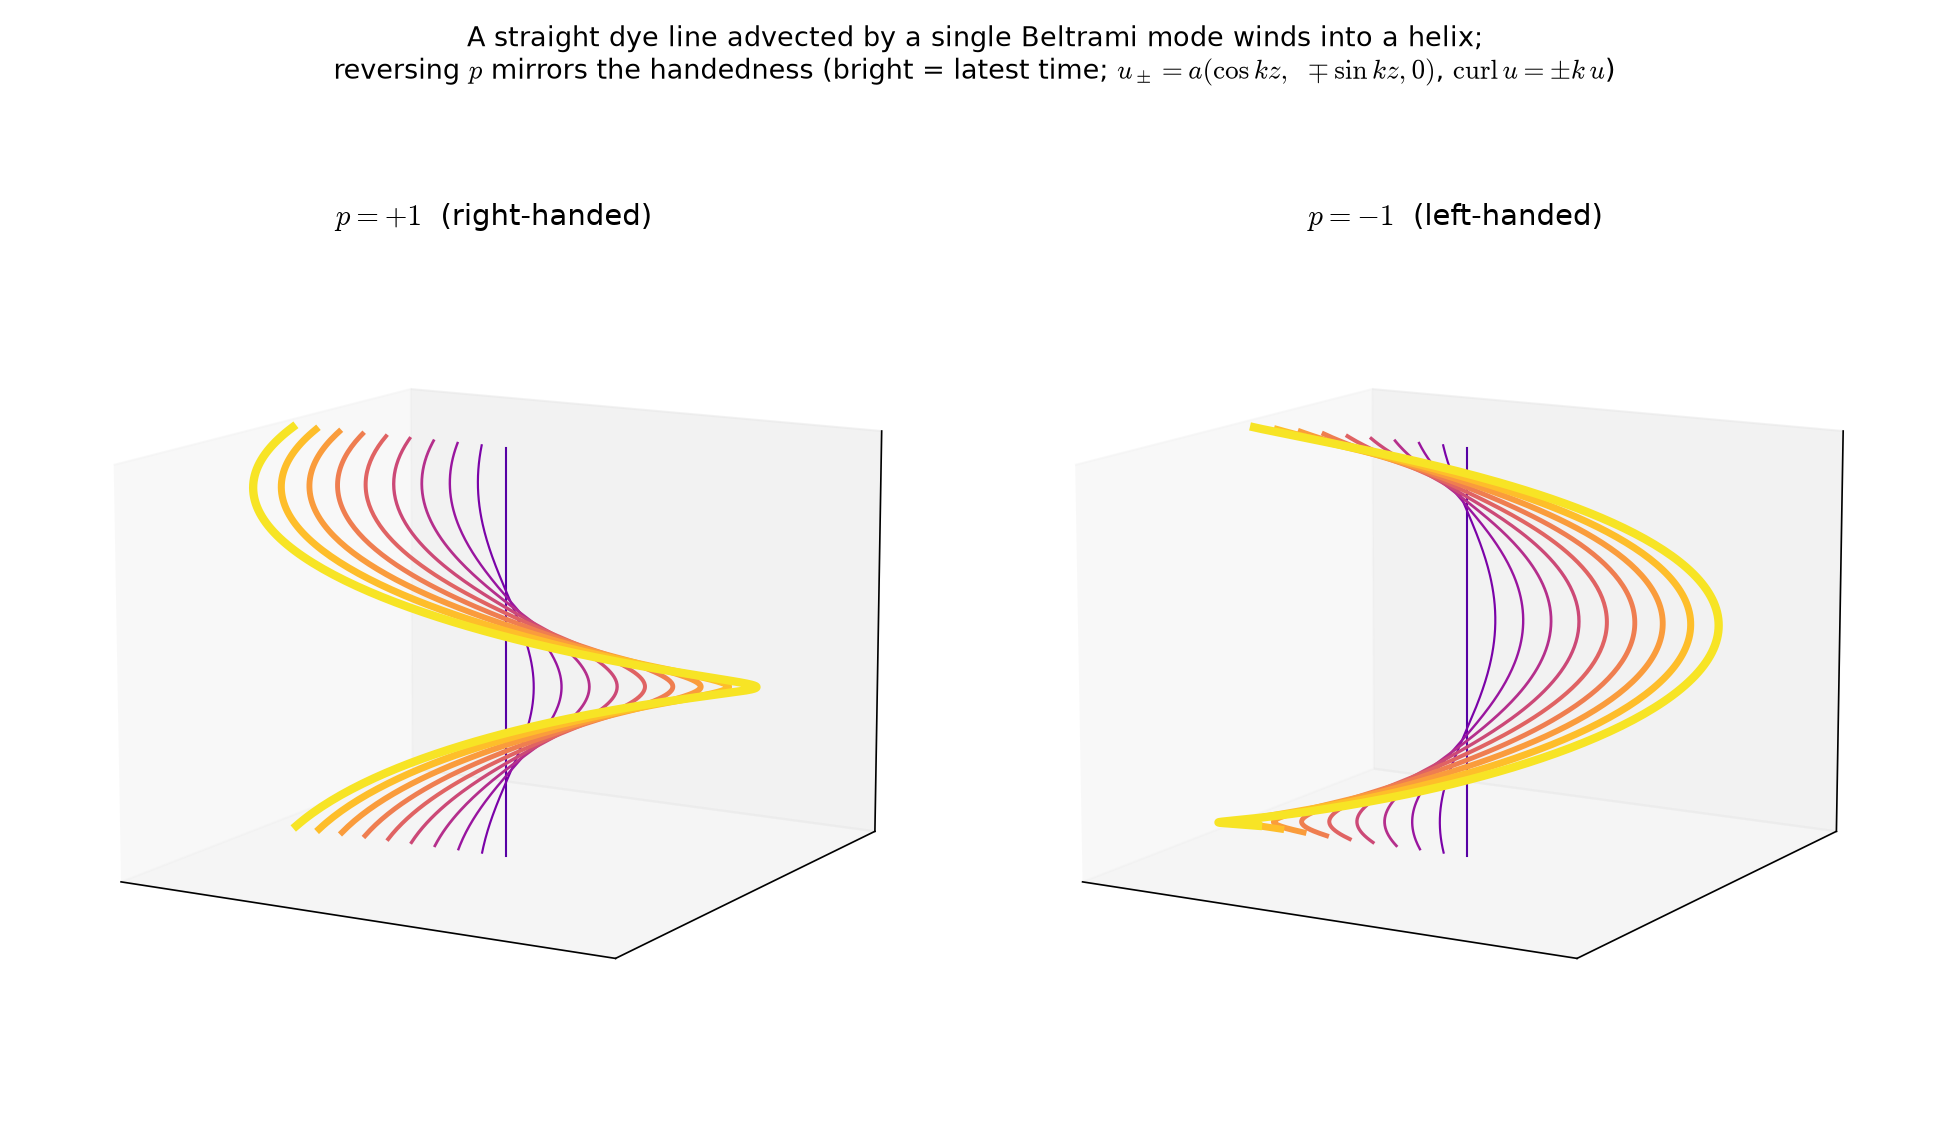
\includegraphics[width=0.92\linewidth]{figures/helix.png}
  \caption{The chirality made concrete on a single Beltrami mode
    $\bu(\bx)=a(\cos kz,\mp\sin kz,0)$, which satisfies $\curl\bu=\pm k\,\bu$
    (the real-space, single-$\bk$ realization of the helical basis
    of~\eqref{eq:helical}). A straight dye line (dark) advected by the field winds
    into a one-turn helix (bright is the latest time); reversing the sign of $p$
    mirrors the handedness exactly. This is the single-shell limit in which
    $|\rho|=1$; a multi-shell spectrum superposes many such windings, and the net
    $\int\bu\cdot\bomega$ tracks $p$ in sign and magnitude ($+8.5\cdot10^{-4}$ at
    $p=+1$, $-8.6\cdot10^{-4}$ at $p=-1$, $\approx0$ at $p=0$ on a $32^3$ grid).}
  \label{fig:helix}
\end{figure}

A scale-independent readout of the effect is the \emph{relative helicity}
\begin{equation}
\rho \;=\; \frac{\langle \bu\cdot\bomega\rangle}{\sqrt{\langle|\bu|^2\rangle}\,
\sqrt{\langle|\bomega|^2\rangle}} \;\in[-1,1],
\label{eq:rho}
\end{equation}
with $\rho=\pm1$ only for a single-shell Beltrami field. For a spectrum spanning many shells,
$|\rho|<1$ even at $p=\pm1$, because $\bu$ and $\bomega$ cannot be pointwise parallel across
scales simultaneously; \S\ref{sec:validation} measures this ceiling.

\FloatBarrier
\section{Real fields and preservation of the helicity bias}
\label{sec:hermitian}

Why this section matters to a practitioner: assembling the field from complex waves is
convenient, but a velocity field you can actually advect through must be real-valued, and the
standard step that makes it real pairs up opposite waves in a way that could, in principle,
quietly cancel the left/right bias the artist just dialled in. It does not. The handedness
survives that step exactly---the dial you set is the dial you get---and the rest of this section
proves it. A reader who is content to take that on faith can skip to \S\ref{sec:coherence}.

In detail: building modes with complex amplitudes yields a complex
field; the standard remedy is to impose Hermitian symmetry
$\hat\bu(-\bk)=\overline{\hat\bu(\bk)}$, after which the inverse transform is exactly real.
The nontrivial question is whether this symmetrization, which couples each $+\bk$ mode to its
$-\bk$ partner, preserves the helicity bias~\eqref{eq:split} or averages it away. It preserves
it.

\begin{proposition}\label{prop:pres}
Adopt the antipodal frame convention $\ehat_1(-\bk)=\ehat_1(\bk)$,
$\ehat_2(-\bk)=-\ehat_2(\bk)$ (which keeps $\{\ehat_1,\ehat_2,\khat\}$ right-handed at
$-\bk$). Then
\begin{equation}
\he_+(-\bk) = \overline{\he_+(\bk)} = \he_-(\bk),
\label{eq:parity}
\end{equation}
and imposing $\hat\bu(-\bk)=\overline{\hat\bu(\bk)}$ forces the helical amplitudes at $-\bk$
to be $a_\pm(-\bk)=\overline{a_\pm(\bk)}$. In particular $|a_+(-\bk)|=|a_+(\bk)|$: positive-
and negative-helicity energy are each conserved, and the helicity of the realized real field
is exactly $\mathcal H = 2\sum_{\bk\in H}|\bk|(|a_+(\bk)|^2-|a_-(\bk)|^2)$ over a spectral
half-space $H$ (exact per realization, as the symmetrization conjugates only phases), i.e.\
the bias~\eqref{eq:split} survives verbatim.
\end{proposition}

The proof is a short two-line computation on the helical parity relation~\eqref{eq:parity};
it, together with the frame-convention and Nyquist-plane implementation notes, is deferred to
Appendix~\ref{app:hermitian}. The practical upshot is all that the construction needs:
assemble $\hat\bu(\bk)$ on a spectral half-space and set
$\hat\bu(-\bk)=\overline{\hat\bu(\bk)}$, and the handedness bias comes through untouched.

\FloatBarrier
\section{Phase coherence at fixed spectrum}
\label{sec:coherence}

This is the organization dial. Picture the same amount of motion at every scale---the flow is
neither faster nor slower, finer nor coarser---but arranged two different ways: as an even,
directionless haze, or gathered into a few distinct rolling vortices. What separates the two is
not \emph{how much} energy each scale carries but whether the waves at different scales line up
in phase. This dial slides between those two arrangements while leaving the per-scale energy
untouched, so the flow visibly reorganizes without changing pace. Curl-noise has no equivalent:
its arrangement is whatever its potential happened to give.

The power spectrum $|\hat\bu(\bk)|^2$ fixes how much energy sits at each scale; it says nothing
about how the modes are \emph{aligned} in phase. A field whose inter-mode phases are
independent and uniform (the random-phase approximation, RPA) is Gaussian and spatially
featureless; introducing correlations among the phases concentrates energy into localized
coherent structures. That structural information lives in the phases rather than the amplitude
spectrum is a standard observation~\cite{coles2000}.

We expose this as a control. Let $c_\lambda(\bk)$ be a \emph{common} unit-modulus complex
scalar applied to all components of a mode, $\hat\bu(\bk)\mapsto c_\lambda(\bk)\hat\bu(\bk)$.
Because the multiplier is common to the vector's three components, it cancels in the one-point
spectral tensor $\Phi_{ab}(\bk)=\hat u_a\overline{\hat u_b}$ (the factor $|c_\lambda|^2=1$
drops out), so the power spectrum \emph{and} the helical polarization~\eqref{eq:split} are
frozen \emph{exactly} at every $\lambda$; and with an antisymmetric phase
$\theta(-\bk)=-\theta(\bk)$ the field stays real and divergence-free. Two convenient families,
with $\theta(\bk)$ drawn uniformly on a spectral half-space and $\lambda\in[0,1]$:
\begin{align}
\text{(linear)}\quad & c_\lambda(\bk)=\exp\!\big(i(1-\lambda)\,\theta(\bk)\big),
\label{eq:schemeA}\\[2pt]
\text{(chord)}\quad & c_\lambda(\bk)=\frac{\lambda+(1-\lambda)e^{i\theta(\bk)}}
{\big|\lambda+(1-\lambda)e^{i\theta(\bk)}\big|}.
\label{eq:schemeB}
\end{align}
At $\lambda=1$ the phases are those of a chosen structured reference; at $\lambda=0$ they are
i.i.d.\ random (the RPA surrogate of the same amplitudes). Sliding $\lambda$ carries the field
from formless noise to organized filaments \emph{without changing the energy at any scale} ---
the axis that curl-noise lacks. (In the demonstrations of \S\ref{sec:validation} the reference
phases are those of a sparse set of localized vortex ``blobs'', so raising $\lambda$ grows
distinct rolling vortices out of the haze.) Figure~\ref{fig:curlnoise} shows the two ends of
this axis side by side at a fixed spectrum: the $\lambda=0$ field is the featureless Gaussian
haze that curl-noise produces, while $\lambda=1$ pulls the same energy into distinct coherent
vortices.

\FloatBarrier
\section{A real-time analytic variant}
\label{sec:modesum}

The two evaluation paths compute the same kind of field but serve opposite use cases, and the
choice between them is a practical one. The FFT bake (\S\ref{sec:construction}) fills a full,
dense spectrum on a grid once, then hands downstream animation a static texture---richest detail
and exact tiling, but a per-rebuild cost, so it is the offline authoring tool. The mode-sum
below sums a sparse handful of analytic waves and evaluates the field at any single point on
demand, with no grid and no transform---cheaper to re-evaluate and resolution-independent, at
the price of sparser detail and only approximate tiling, which is what makes it the real-time,
in-shader option. They are not merely two implementations of one routine: the FFT path is dense
and grid-baked, the mode-sum path is sparse and pointwise, and \S\ref{sec:validation}
(E3, E5) quantifies both the cost split and the one behavioural difference it introduces (a
small residual handedness at $p=0$). Use the FFT bake when authoring a hero field offline; use
the mode-sum when the field must be evaluated live.

The FFT construction pays an $N^d$ transform per rebuild---bake-scale, not real-time. An
alternative sums a sparse set of analytic helical modes and evaluates the field \emph{per
point}, with no grid and no transform:
\begin{equation}
\bu(\bx)=\sum_{j=1}^{N} a_j\big(\ehat_{1,j}\cos\phi_j - s_j\,\ehat_{2,j}\sin\phi_j\big),
\qquad \phi_j=\bk_j\cdot\bx+\theta_j,
\label{eq:modesum}
\end{equation}
with directions $\khat_j$ uniform on the sphere, amplitude $a_j=|\bk_j|^{-s}$, transverse
frame $(\ehat_{1,j},\ehat_{2,j})\perp\bk_j$, and per-mode helicity sign $s_j\in\{+1,-1\}$
drawn with $\Pr(s_j=+1)=(1+p)/2$. Each term is the real part of a single helical mode: it is
analytically transverse to its own $\bk_j$, so $\dvg\bu\equiv0$ pointwise, and it is a
Beltrami mode, $\curl\bu_j=s_j|\bk_j|\bu_j$. Consequently the vorticity is a second cheap
mode-sum requiring no derivatives,
$\bomega(\bx)=\sum_j s_j|\bk_j|\big(\ehat_{1,j}\cos\phi_j - s_j\ehat_{2,j}\sin\phi_j\big)$,
which makes~\eqref{eq:modesum} well suited to a fragment shader.

Two properties distinguish~\eqref{eq:modesum} from the FFT field. First, it is exactly
divergence-free for every $N$ (the only nonzero divergence one measures is
finite-difference truncation, \S\ref{sec:validation}). Second---and this is a genuine
caveat---at $p=0$ a \emph{finite} mode set does not cancel helicity exactly: the realized net
helicity is a statistical fluctuation of size $\mathcal O(N^{-1/2})$ about zero, so the slider
value $p$ is only the \emph{intended} bias. An implementation should therefore report the
\emph{measured} net $\bu\cdot\bomega$ rather than $p$. The FFT construction does not share this
caveat because it fills a full shell of modes.

A WebGL2 / GLSL ES 3.0 fragment shader implementing~\eqref{eq:modesum} directly
accompanies the paper (\texttt{code/modesum.frag}): the $M$ modes are uploaded
once as a small $M\times3$ float texture (rows $(\bk,\theta)$, $(\ehat_1,a)$,
$(\ehat_2,s)$, built exactly as \texttt{e3\_mode\_sum.py}), and each pixel runs
the $\mathcal O(M)$ sum. A CPU port of the shader's exact arithmetic is
divergence-free to $\max_j|\bk_j\cdot\ehat_{i,j}|=5.6\cdot10^{-16}$ (the only
nonzero divergence measured is $\mathcal O(h^2)$ finite-difference truncation),
matching~E3.

\FloatBarrier
\section{Solid obstacles}
\label{sec:obstacles}

In plain terms: we want the flow to slide around a solid object---a rock, a
character, a wall---without ever leaking into it, and without running a fluid
solver to enforce that. The usual worry is that clamping a velocity field near a
wall reintroduces the very compression the divergence-free construction was meant
to avoid. The trick that avoids this is to damp the field's \emph{potential}
rather than the field itself, and only then take the curl: because the result is
a curl, it is divergence-free by the same identity $\dvg\curl\equiv0$ that
underlies curl-noise, \emph{for any obstacle and any damping profile}.

Concretely, every field of this paper has an analytic vector potential $\bA$
($\curl\bA=\bu$): on the helical basis each mode is a curl eigenvector
\eqref{eq:eigen}, so $\bA=\sum_\bk (a_+\he_+ + a_-\he_-)/(\pm|\bk|)$, and for the
mode-sum \eqref{eq:modesum} the potential is the term-by-term
$\bA=\sum_j \bu_j/(s_j|\bk_j|)$. Given a solid described by a signed-distance
function $d(\bx)$ (positive outside, zero on the surface), we fade the potential
to zero across a thin band of thickness $\theta$ with a smooth ramp $\alpha$ of
the distance and take the curl of the faded potential:
\begin{equation}
\bu_b(\bx) \;=\; \curl\!\big(\alpha(d/\theta)\,\bA\big)
\;=\; \tfrac{1}{\theta}\,\alpha'(d/\theta)\,\big(\nabla d\times\bA\big)
\;+\; \alpha(d/\theta)\,\bu ,
\label{eq:bounded}
\end{equation}
using $\curl(f\bA)=\nabla f\times\bA + f\,\curl\bA$. The ramp is the
Bridson curl-noise boundary quintic~\cite{bridson2007},
\begin{equation}
\alpha(q)=\tfrac{1}{8}\,q\,(15-10q^2+3q^4)\ \ \text{on }[0,1],\qquad
\alpha(q\le0)=0,\ \ \alpha(q\ge1)=1,
\label{eq:quintic}
\end{equation}
with $\alpha(0)=0$ but $\alpha'(0)=\tfrac{15}{8}>0$, so the wall value is a pure
tangential slip flow rather than a no-slip dead zone, and $\alpha(1)=1$ with
$\alpha'(1)=\alpha''(1)=0$, so the field blends $C^2$-smoothly back into the
unconstrained one at the edge of the band (Fig.~\ref{fig:ramp}). Inside the solid
($d\le0$) the field is identically zero.

\begin{figure}[htbp]
  \centering
  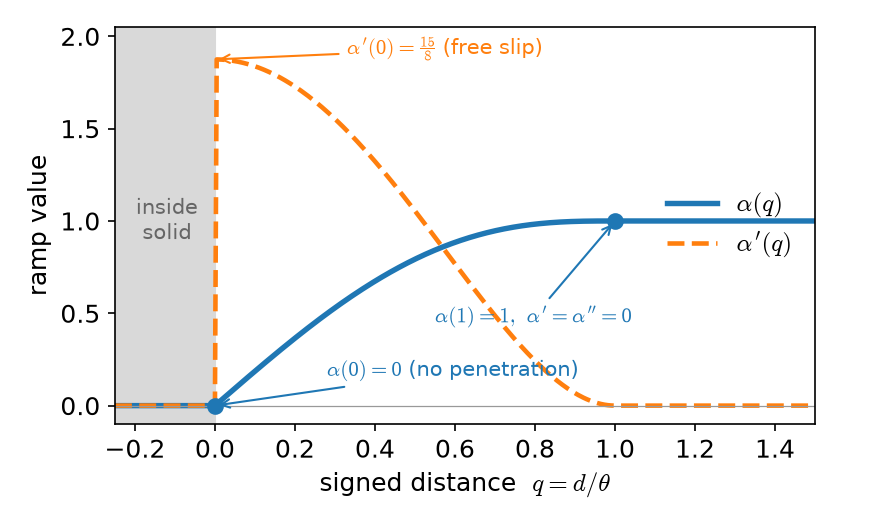
\includegraphics[width=0.62\linewidth]{figures/ramp.png}
  \caption{The Bridson free-slip quintic~\eqref{eq:quintic} used to fade the
    vector potential across the obstacle band. The ramp $\alpha$ (solid) rises
    from $0$ at the wall to $1$ at the band edge; its derivative $\alpha'$ (dashed)
    is nonzero at the wall ($\alpha'(0)=\tfrac{15}{8}$, giving tangential slip
    rather than a dead zone) and vanishes to second order at the edge, so the
    bounded field meets the unconstrained one $C^2$-smoothly. The distance is
    normalized by the band thickness, $q=d/\theta$.}
  \label{fig:ramp}
\end{figure}

Two properties hold \emph{by construction}, independent of the ramp or the
obstacle shape. First, $\bu_b$ is exactly divergence-free everywhere: it is a
curl. Second, it is tangent to the surface: on the surface $d=0$, the first term
of~\eqref{eq:bounded} carries the factor $\nabla d\times\bA$, whose component
along the surface normal $\hat\bn=\nabla d$ is $(\nabla d\times\bA)\cdot\nabla d=0$
identically, while the second term carries the factor $\alpha(0)=0$; hence
$\bu_b\cdot\hat\bn=0$ on the wall. This is precisely the free-slip,
boundary-respecting behaviour targeted by pointwise incompressible interpolation
for grid-based fluids~\cite{chang2022}, obtained here in closed form on the
analytic field with no grid and no projection. Beyond the band ($d\ge\theta$) the
field is bit-identical to the unconstrained one.

\paragraph{(E6) Obstacle: tangency, containment, and machine-zero divergence
  \textnormal{(\texttt{e6\_obstacle.py})}.}
We place a sphere of radius $R=1$ in the mode-sum field ($N=40$ modes, slope
$s=1$, band $\theta=0.6$, pinned seed) and measure the three guarantees
(Fig.~\ref{fig:obstacle}). \textbf{(a) Tangency:} over $20{,}000$ surface points
the peak normal flux relative to the rms speed is
$\max|\bu_b\cdot\hat\bn|/\mathrm{rms}|\bu_b| = 4.8\cdot10^{-16}$---machine zero,
the free-slip guarantee holding exactly. \textbf{(b) Containment:} advecting
$5000$ tracer particles seeded in and around the influence band through the steady
field with RK4, the fraction that end up \emph{inside} the sphere is $0.00\%$ with
the ramp against $2.84\%$ without it (raw field), matching the independent GPU
particle-readback figure of $0$ versus ${\approx}2.9\%$. \textbf{(c) Divergence:}
$\bu_b$ is an analytic curl, so $\dvg\bu_b=0$ identically; symbolic algebra
confirms $\dvg\curl(f\bA)=0$, and a complex-step evaluation of the analytic
divergence in the band interior gives rms $1.2\cdot10^{-15}$ (machine zero),
whereas a naive central-difference stencil at $h=0.01$ reports rms
$7.2\cdot10^{-4}$---the $\mathcal O(h^2)$ truncation of the stencil, not an error
in the field. Every number here is emitted by \texttt{e6\_obstacle.py}.

\begin{figure}[htbp]
  \centering
  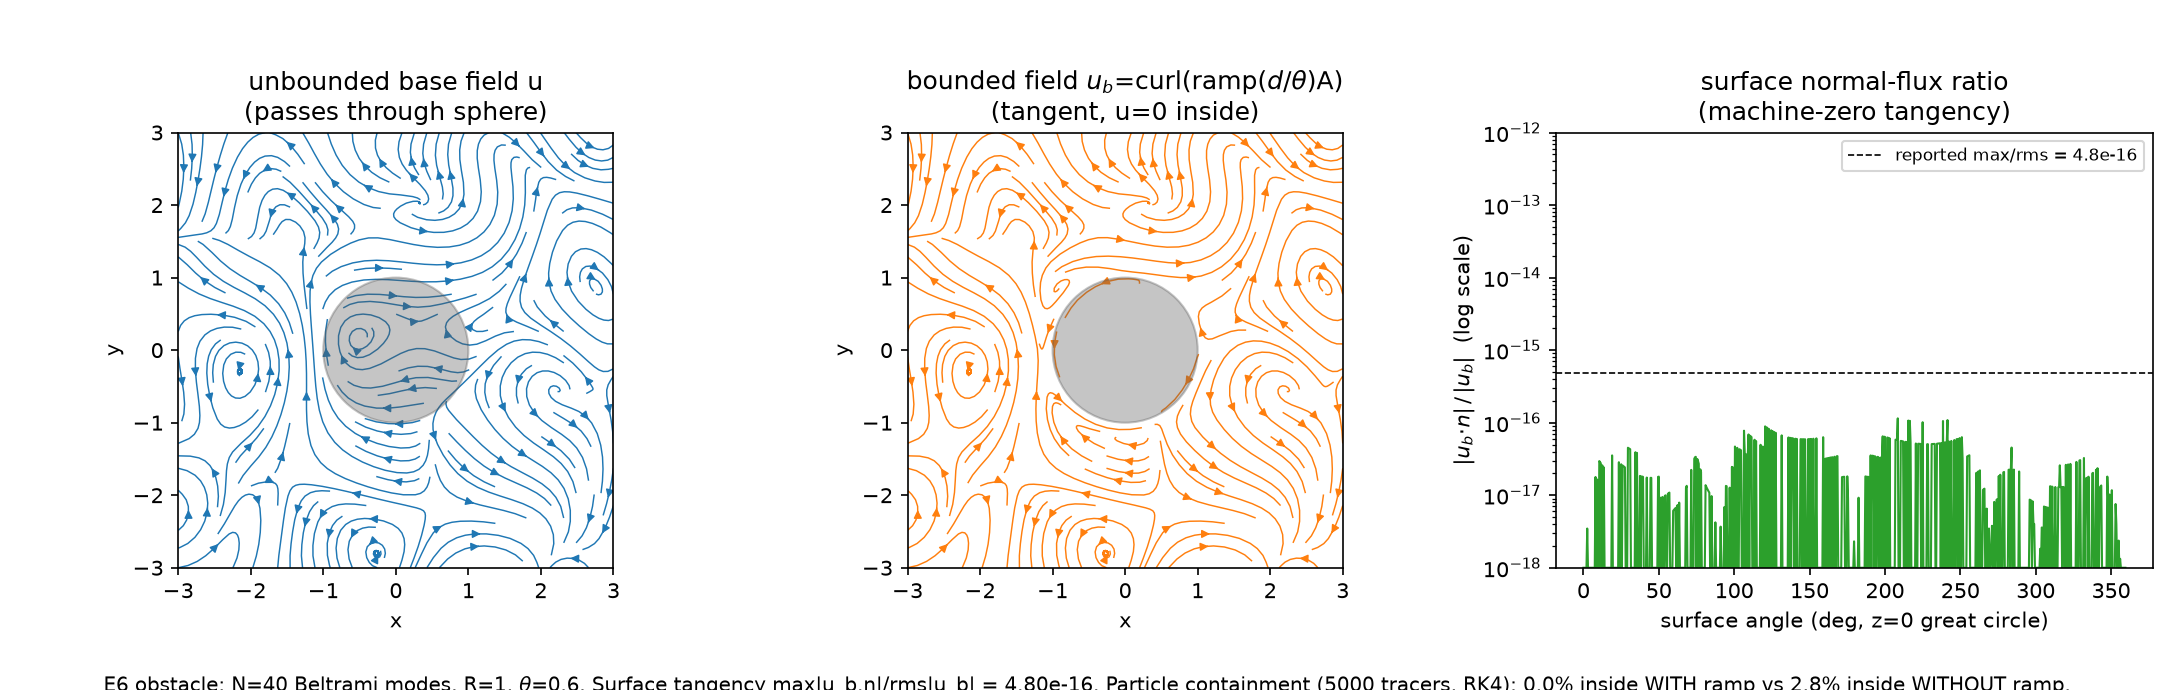
\includegraphics[width=\linewidth]{figures/obstacle.png}
  \caption{Solid-obstacle handling by ramping the vector potential before the
    curl~\eqref{eq:bounded}. \textbf{Left:} the unconstrained field passes
    straight through the sphere. \textbf{Middle:} the bounded field
    $\bu_b=\curl(\alpha(d/\theta)\bA)$ bends tangentially around it and is zero
    inside---exactly divergence-free because it is a curl, and free-slip because
    $\alpha(0)=0$. \textbf{Right:} the surface normal-flux ratio
    $|\bu_b\cdot\hat\bn|/|\bu_b|$ at points around the sphere sits at machine zero
    ($\max/\mathrm{rms}=4.8\cdot10^{-16}$). Of $5000$ advected particles, $0.00\%$
    finish inside the sphere with the ramp versus $2.84\%$ without it
    (\texttt{e6\_obstacle.py}, sphere $R=1$, $N=40$ modes, band $\theta=0.6$).}
  \label{fig:obstacle}
\end{figure}

\FloatBarrier
\section{Numerical validation}
\label{sec:validation}

We report five experiments (E1--E5), each reproduced by a self-contained script accompanying
the paper (\texttt{code/e1\_*..e5\_*}); the obstacle experiment E6 is reported in
\S\ref{sec:obstacles} (\texttt{code/e6\_obstacle.py}). The printed numbers below are exactly
those the scripts emit at the pinned seed.

\paragraph{(E1) Helical identities \textnormal{(\texttt{e1\_helical\_identities.py})}.}
Over $2000$ random real wavevectors, the transversality and curl-eigenvector
relations~\eqref{eq:eigen} hold to $\|\he_\pm\cdot\bk\|\le 4.1\cdot10^{-16}$ and
$\|i\bk\times\he_\pm\mp|\bk|\he_\pm\|\le1.0\cdot10^{-15}$; in symbolic algebra both are
identically zero. The parity identity~\eqref{eq:parity} holds \emph{exactly} (residual $0$),
and the amplitude map of Proposition~\ref{prop:pres} to $2.4\cdot10^{-15}$ numerically and
exactly in symbolic algebra.

\paragraph{(E2) FFT field: real, divergence-free, helicity linear in $p$
\textnormal{(\texttt{e2\_fft\_field.py})}.}
On a $32^3$ grid with slope $s=1.6$, enforcing Hermitian symmetry:
\begin{center}
\begin{tabular}{rccc}
\toprule
$p$ & $\max|\bk\cdot\hat\bu|/|\hat\bu|$ & $\max|\mathrm{Im}\,\bu|$ & $\rho$\\
\midrule
$-1.0$ & $4.4\cdot10^{-17}$ & $4.7\cdot10^{-20}$ & $-0.7961$\\
$-0.5$ & $6.3\cdot10^{-17}$ & $4.9\cdot10^{-20}$ & $-0.3981$\\
$\phantom{-}0.0$ & $5.8\cdot10^{-17}$ & $5.3\cdot10^{-20}$ & $\phantom{-}0.0000$\\
$\phantom{-}0.5$ & $5.8\cdot10^{-17}$ & $4.9\cdot10^{-20}$ & $\phantom{-}0.3981$\\
$\phantom{-}1.0$ & $4.4\cdot10^{-17}$ & $5.4\cdot10^{-20}$ & $\phantom{-}0.7961$\\
\bottomrule
\end{tabular}
\end{center}
The field is divergence-free and real to machine precision, and $\rho$ is linear in $p$ (fit
$\rho=0.79612\,p$, maximum deviation from the line $1.1\cdot10^{-16}$), zero at $p=0$, and
correct in sign. The ceiling $|\rho(\pm1)|\approx0.80$ is below $1$ because the spectrum spans
many shells; it is spectrum-dependent ($\rho(+1)=0.821,\,0.796,\,0.812$ at slopes
$s=1.2,\,1.6,\,2.0$), consistent with the single-shell remark after~\eqref{eq:rho}.

\paragraph{(E3) Mode-sum: exact transversality and the $N^{-1/2}$ helicity residual
\textnormal{(\texttt{e3\_mode\_sum.py})}.}
For~\eqref{eq:modesum} the analytic transversality is machine-exact,
$\max_j|\bk_j\cdot\ehat_{i,j}|=4.4\cdot10^{-16}$, so $\dvg\bu=0$ analytically; the
central-difference divergence falls cleanly as $\mathcal O(h^2)$ (rms
$2.6\cdot10^{-2}\to4.1\cdot10^{-4}$ as $h$ halves from $0.1$, Richardson ratios
$3.96,3.99,4.00$), confirming truncation rather than construction error. With $N=40$ modes,
$\rho(p)=(-0.889,-0.662,+0.069,+0.383,+0.888)$ for $p=(-1,-\tfrac12,0,\tfrac12,1)$, monotone
and saturating near $\pm1$; the $+0.069$ at $p=0$ is one draw's grid-measured relative
helicity, a realization of the finite-$N$ fluctuation. To exhibit its decay we use the
$|\bk|$-weighted net-helicity estimator
$h_N:=\big(\textstyle\sum_j s_j|\bk_j|a_j^2\big)\big/\big(\sum_j|\bk_j|a_j^2\big)$, whose
mean is $p$; averaged over $200$ draws at $p=0$,
\[
\mathrm{rms}\,h_N \;=\; 0.253,\,0.176,\,0.114,\,0.090,\,0.064
\quad\text{for } N=20,40,80,160,320,
\]
i.e.\ $\mathrm{rms}\,h_N\cdot\sqrt N\approx1.0$--$1.14$ (fitted exponent $-0.494$ vs.\ the
predicted $-\tfrac12$), the $\mathcal O(N^{-1/2})$ fluctuation of \S\ref{sec:modesum}. (The
grid-measured $\rho$ and $h_N$ are two $\mathcal O(N^{-1/2})$ proxies for the same finite-$N$
net helicity.) Figure~\ref{fig:validation} plots both results.

\begin{figure}[htbp]
  \centering
  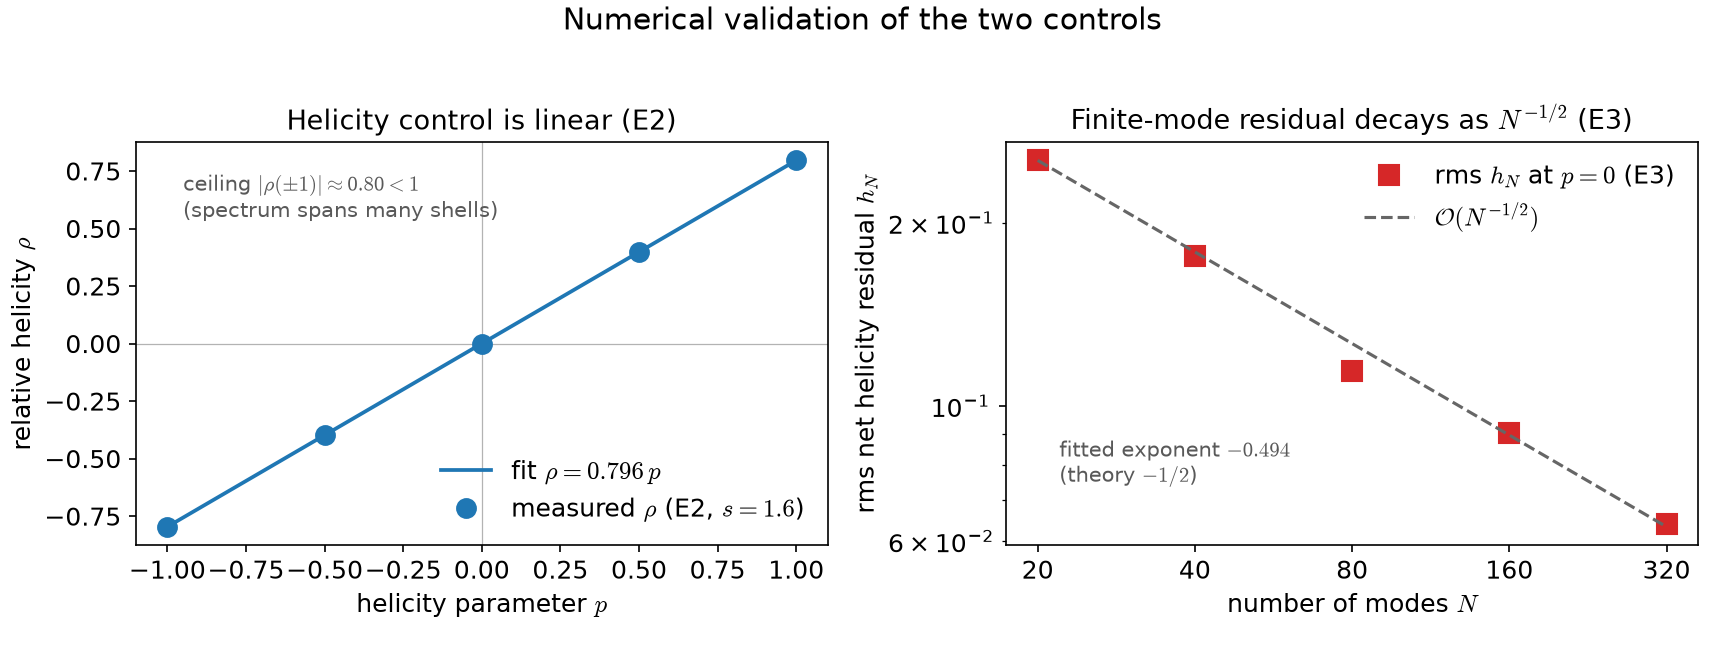
\includegraphics[width=\linewidth]{figures/validation.png}
  \caption{The two quantitative results of E2 and E3. \textbf{Left:} for the FFT
    field the relative helicity $\rho$ is linear in the knob $p$ (fit
    $\rho=0.796\,p$); the ceiling $|\rho(\pm1)|\approx0.80<1$ reflects a spectrum
    spanning many shells~\eqref{eq:rho}. \textbf{Right:} for the mode-sum, the
    net-helicity residual at $p=0$ decays as $\mathcal O(N^{-1/2})$ with mode count
    (fitted exponent $-0.494$), the finite-$N$ fluctuation of \S\ref{sec:modesum}.}
  \label{fig:validation}
\end{figure}

\paragraph{(E4) Phase coherence freezes the spectrum while changing structure
  \textnormal{(\texttt{e4\_phase\_coherence.py})}.}
The phase-coherence axis (\S\ref{sec:coherence}) claims to move the field from
formless noise to organized filaments \emph{without touching the energy at any
scale}. We verify both halves on the 2D construction ($160^2$ grid, slope
$s=1.4$). As the coherence knob $\lambda$ is swept $0\to1$ under scheme~A
\eqref{eq:schemeA}, the total spectral energy is invariant to
$\sum|\hat\bu|^2 = 5.209353$ at every $\lambda$ (spread $1.8\cdot10^{-15}$,
relative $3.4\cdot10^{-16}$), and the per-shell energy spectrum is likewise
frozen (maximum relative deviation of any shell across $\lambda$ is
$2.7\cdot10^{-16}$); the field stays divergence-free
($\max|\bk\cdot\hat\bu|/|\hat\bu|\le1.4\cdot10^{-17}$) and real
($\max|\mathrm{Im}\,\bu|\sim10^{-7}$, at rounding). The spatial organization,
by contrast, changes monotonically: the flatness (kurtosis) of the vorticity,
which is $3$ for a Gaussian random-phase field and grows as energy concentrates
into sparse coherent structures, rises
\[
  \mathrm{flatness}(\omega)\;=\;3.13,\;3.93,\;5.79,\;8.20,\;9.22
  \qquad\text{for }\lambda=0,\,0.25,\,0.5,\,0.75,\,1
\]
(16-draw mean), from the Gaussian value at $\lambda=0$ up to strongly
intermittent at $\lambda=1$. Structure appears; energy per scale does not move.

\paragraph{(E5) The two cost regimes \textnormal{(\texttt{e5\_performance.py})}.}
The two constructions occupy different cost budgets, whose scaling
Fig.~\ref{fig:perf} measures (single-machine CPU \texttt{numpy} reference; the
scaling is the claim, absolute times are machine-dependent). The FFT path is a
\emph{bake} cost---one $\mathcal O(N^3\log N)$ rebuild per authored field, after
which the field is a static texture ($3.0$\,MB of \texttt{float32} \texttt{vec3}
at $64^3$) and advection downstream is free. The mode-sum path trades the grid for
an $\mathcal O(M)$ per-point evaluation whose throughput falls as $1/M$; the
arithmetic is embarrassingly parallel across pixels, which is why the
fragment-shader implementation (\texttt{code/modesum.frag}), not a scalar CPU loop,
is the real-time target.

\begin{figure}[htbp]
  \centering
  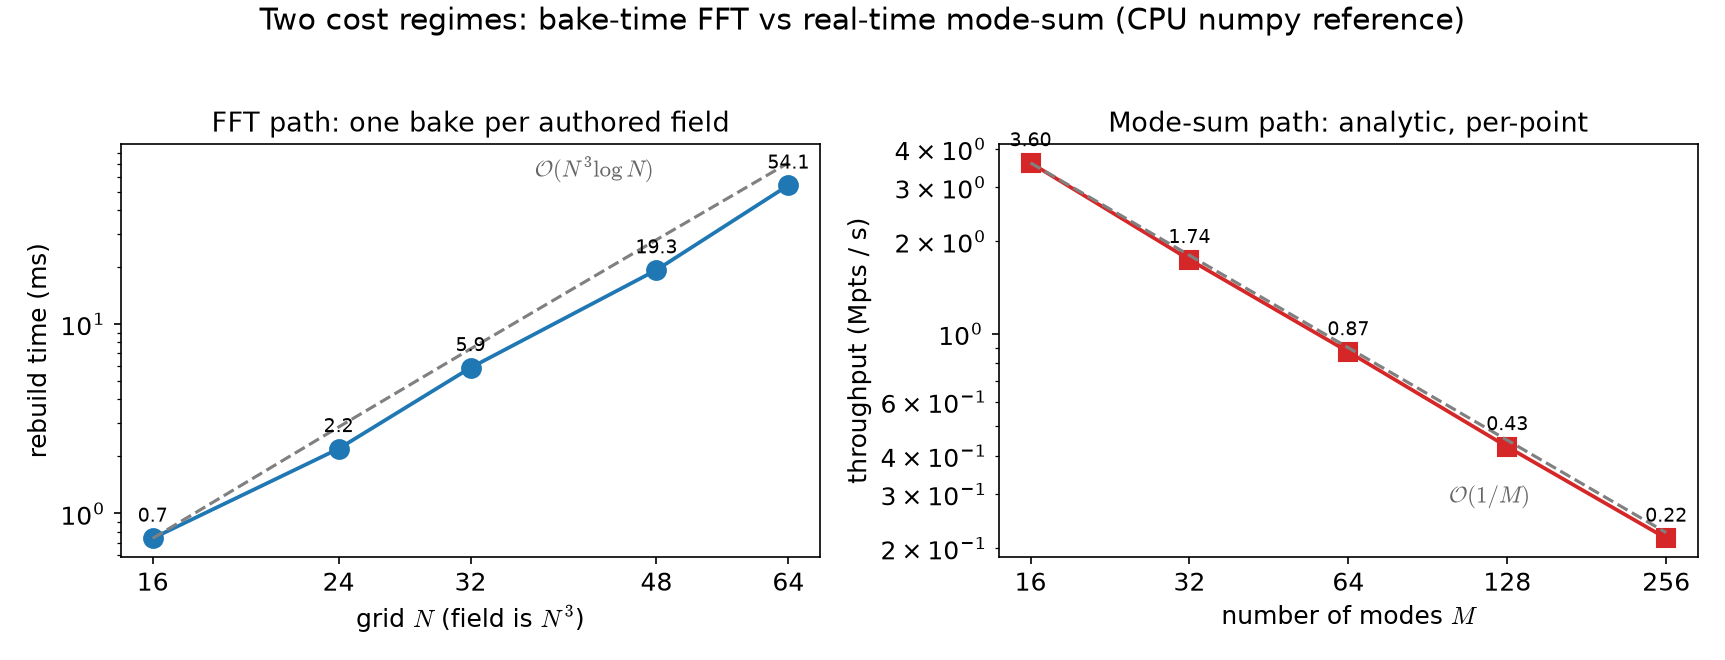
\includegraphics[width=\linewidth]{figures/performance.png}
  \caption{Two cost regimes (CPU \texttt{numpy} reference, one machine, no GPU).
    \textbf{Left:} the FFT construction rebuilds an $N^3$ field in
    $\mathcal O(N^3\log N)$; a bake-time cost paid once per authored field.
    \textbf{Right:} the analytic mode-sum evaluates per point at
    $\mathcal O(M)$ for $M$ modes, so throughput scales as $1/M$. The dashed
    lines are the predicted scalings. Absolute mode-sum rates are for a single
    CPU core; the per-pixel arithmetic parallelises directly on a GPU
    (\texttt{code/modesum.frag}).}
  \label{fig:perf}
\end{figure}

\FloatBarrier
\section{Discussion and limitations}
\label{sec:discussion}

\paragraph{Relation to curl-noise.} Curl-noise~\cite{bridson2007} takes a noise
potential in \emph{real} space and returns its curl, divergence-free by the identity
$\dvg\curl\equiv0$; we assemble the field in the \emph{frequency} domain on the helical
basis, divergence-free by transversality $\he_\pm\cdot\bk=0$. The two mechanisms differ in
what they leave free to control (Table~\ref{tab:curlnoise}): curl-noise is fixed once the
potential is chosen---its handedness is not a parameter, and its phases are those of the
potential---whereas the helical representation exposes the $\pm$ polarization split
(helicity, \S\ref{sec:helicity}) and the common per-mode phase (coherence,
\S\ref{sec:coherence}) as continuous knobs. Curl-noise is precisely the isotropic,
random-phase, mirror-symmetric corner of this space: our $\lambda=0$ field is statistically
indistinguishable from it (equal-spectrum speed flatness $\approx2$ for both, versus
$4.0$ at $\lambda=1$; Fig.~\ref{fig:curlnoise}). The FFT path shares curl-noise's per-frame
cost class but not its constant-time \emph{evaluation}; the mode-sum variant
(\S\ref{sec:modesum}) is the real-time offering.

\begin{table}[t]
  \centering
  \small
  \begin{tabular}{@{}lll@{}}
    \toprule
    & \textbf{Curl-noise}~\cite{bridson2007} & \textbf{This work}\\
    \midrule
    Built in            & real space (noise potential) & frequency domain (helical basis)\\
    Div-free because     & $\dvg\curl\equiv0$ & $\he_\pm\cdot\bk=0$ (transversality)\\
    Spectral slope       & yes (potential band) & yes ($E(\bk)$, \eqref{eq:env})\\
    Helicity / chirality & not a control & knob $p\in[-1,1]$ (\S\ref{sec:helicity})\\
    Phase organization   & tied to potential & knob $\lambda\in[0,1]$ at fixed spectrum\\
    Evaluation           & $\mathcal O(1)$ per point & $\mathcal O(N^d\log N)$ rebuild (FFT)\\
                         &                       & or $\mathcal O(M)$ per point (mode-sum)\\
    \bottomrule
  \end{tabular}
  \caption{Curl-noise and the present construction both produce exactly
    divergence-free fields, but by different mechanisms, which is what makes helicity and
    phase organization controllable here and not there. The random-phase, mirror-symmetric,
    isotropic setting of our method reproduces curl-noise (Fig.~\ref{fig:curlnoise}).}
  \label{tab:curlnoise}
\end{table}

\begin{figure}[htbp]
  \centering
  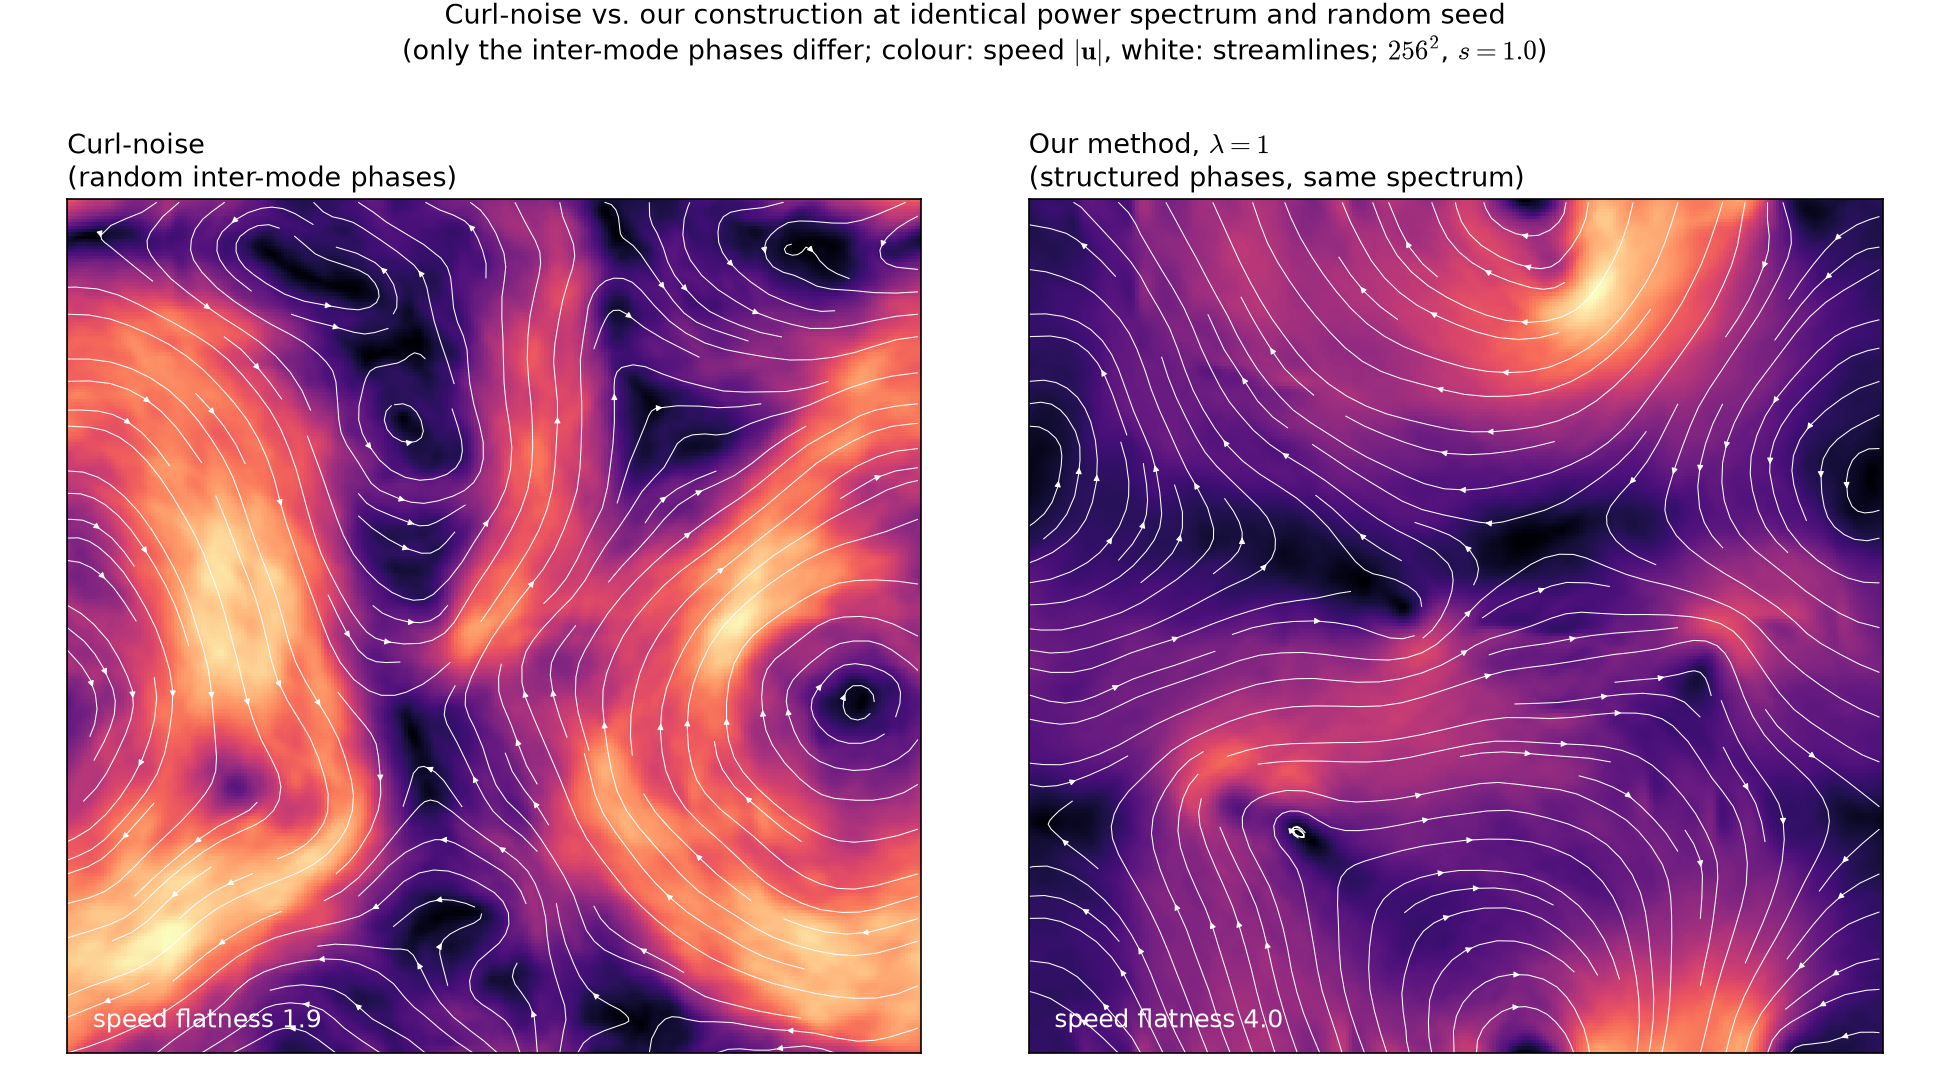
\includegraphics[width=0.92\linewidth]{figures/curlnoise.png}
  \caption{Curl-noise (left) and our construction at $\lambda=1$ (right), built on the
    \emph{same} power spectrum and the same random seed, so that only the inter-mode phases
    differ. Colour is speed $|\bu|$, white curves are streamlines. Curl-noise's random phases
    give a homogeneous field (speed flatness $\approx2$, Gaussian); the structured phases
    concentrate the same energy into distinct coherent vortices (flatness $\approx4$) without
    changing the spectrum---the organization axis curl-noise does not expose.}
  \label{fig:curlnoise}
\end{figure}

\paragraph{Relation to incompressible solvers.} A separate line of graphics work builds
divergence-free fields with explicit vortex and helicity structure inside a time-stepping
\emph{simulator}: Schr\"odinger's smoke~\cite{chern2016} evolves an incompressible field from a
wavefunction, and implicit vortex filaments~\cite{ishida2022} carry controllable vortex
topology; procedural detail is likewise added on top of solvers by guided and stream-guided
synthesis~\cite{kim2008,sato2021} (see~\cite{wang2024} for a recent survey). The present method
is complementary: it is an authoring generator of a static field with no solver and no time
integration, exposing helicity as a continuous polarization knob rather than as an emergent
property of dynamics.

\paragraph{Limits.}
\begin{itemize}[nosep]
\item The FFT path costs an $N^d$ transform per rebuild and is an authoring/bake tool; the
practical deployment bakes the field to a texture or an OpenVDB volume and advects downstream.
\item The mode-sum path is real-time but sparse: it trades away exact tiling and dense-shell
detail, and its $p=0$ state is only mirror-symmetric in the mean ($\mathcal O(N^{-1/2})$
residual, \S\ref{sec:modesum}).
\item The relative-helicity ceiling $|\rho(\pm1)|<1$ is intrinsic to a multi-shell spectrum;
a single-shell field reaches $\pm1$ but looks monochromatic.
\end{itemize}

\paragraph{Applications.} The fields drive the standard procedural pipelines directly
(Fig.~\ref{fig:advection}):
particle advection, semi-Lagrangian smoke density, and volume raymarching of an advected
scalar. Because the field is divergence-free by construction, this transport needs no pressure
projection---the expensive step of a fluid solver---so the two new controls come at no
run-time cost to the downstream renderer.

\begin{figure}[htbp]
  \centering
  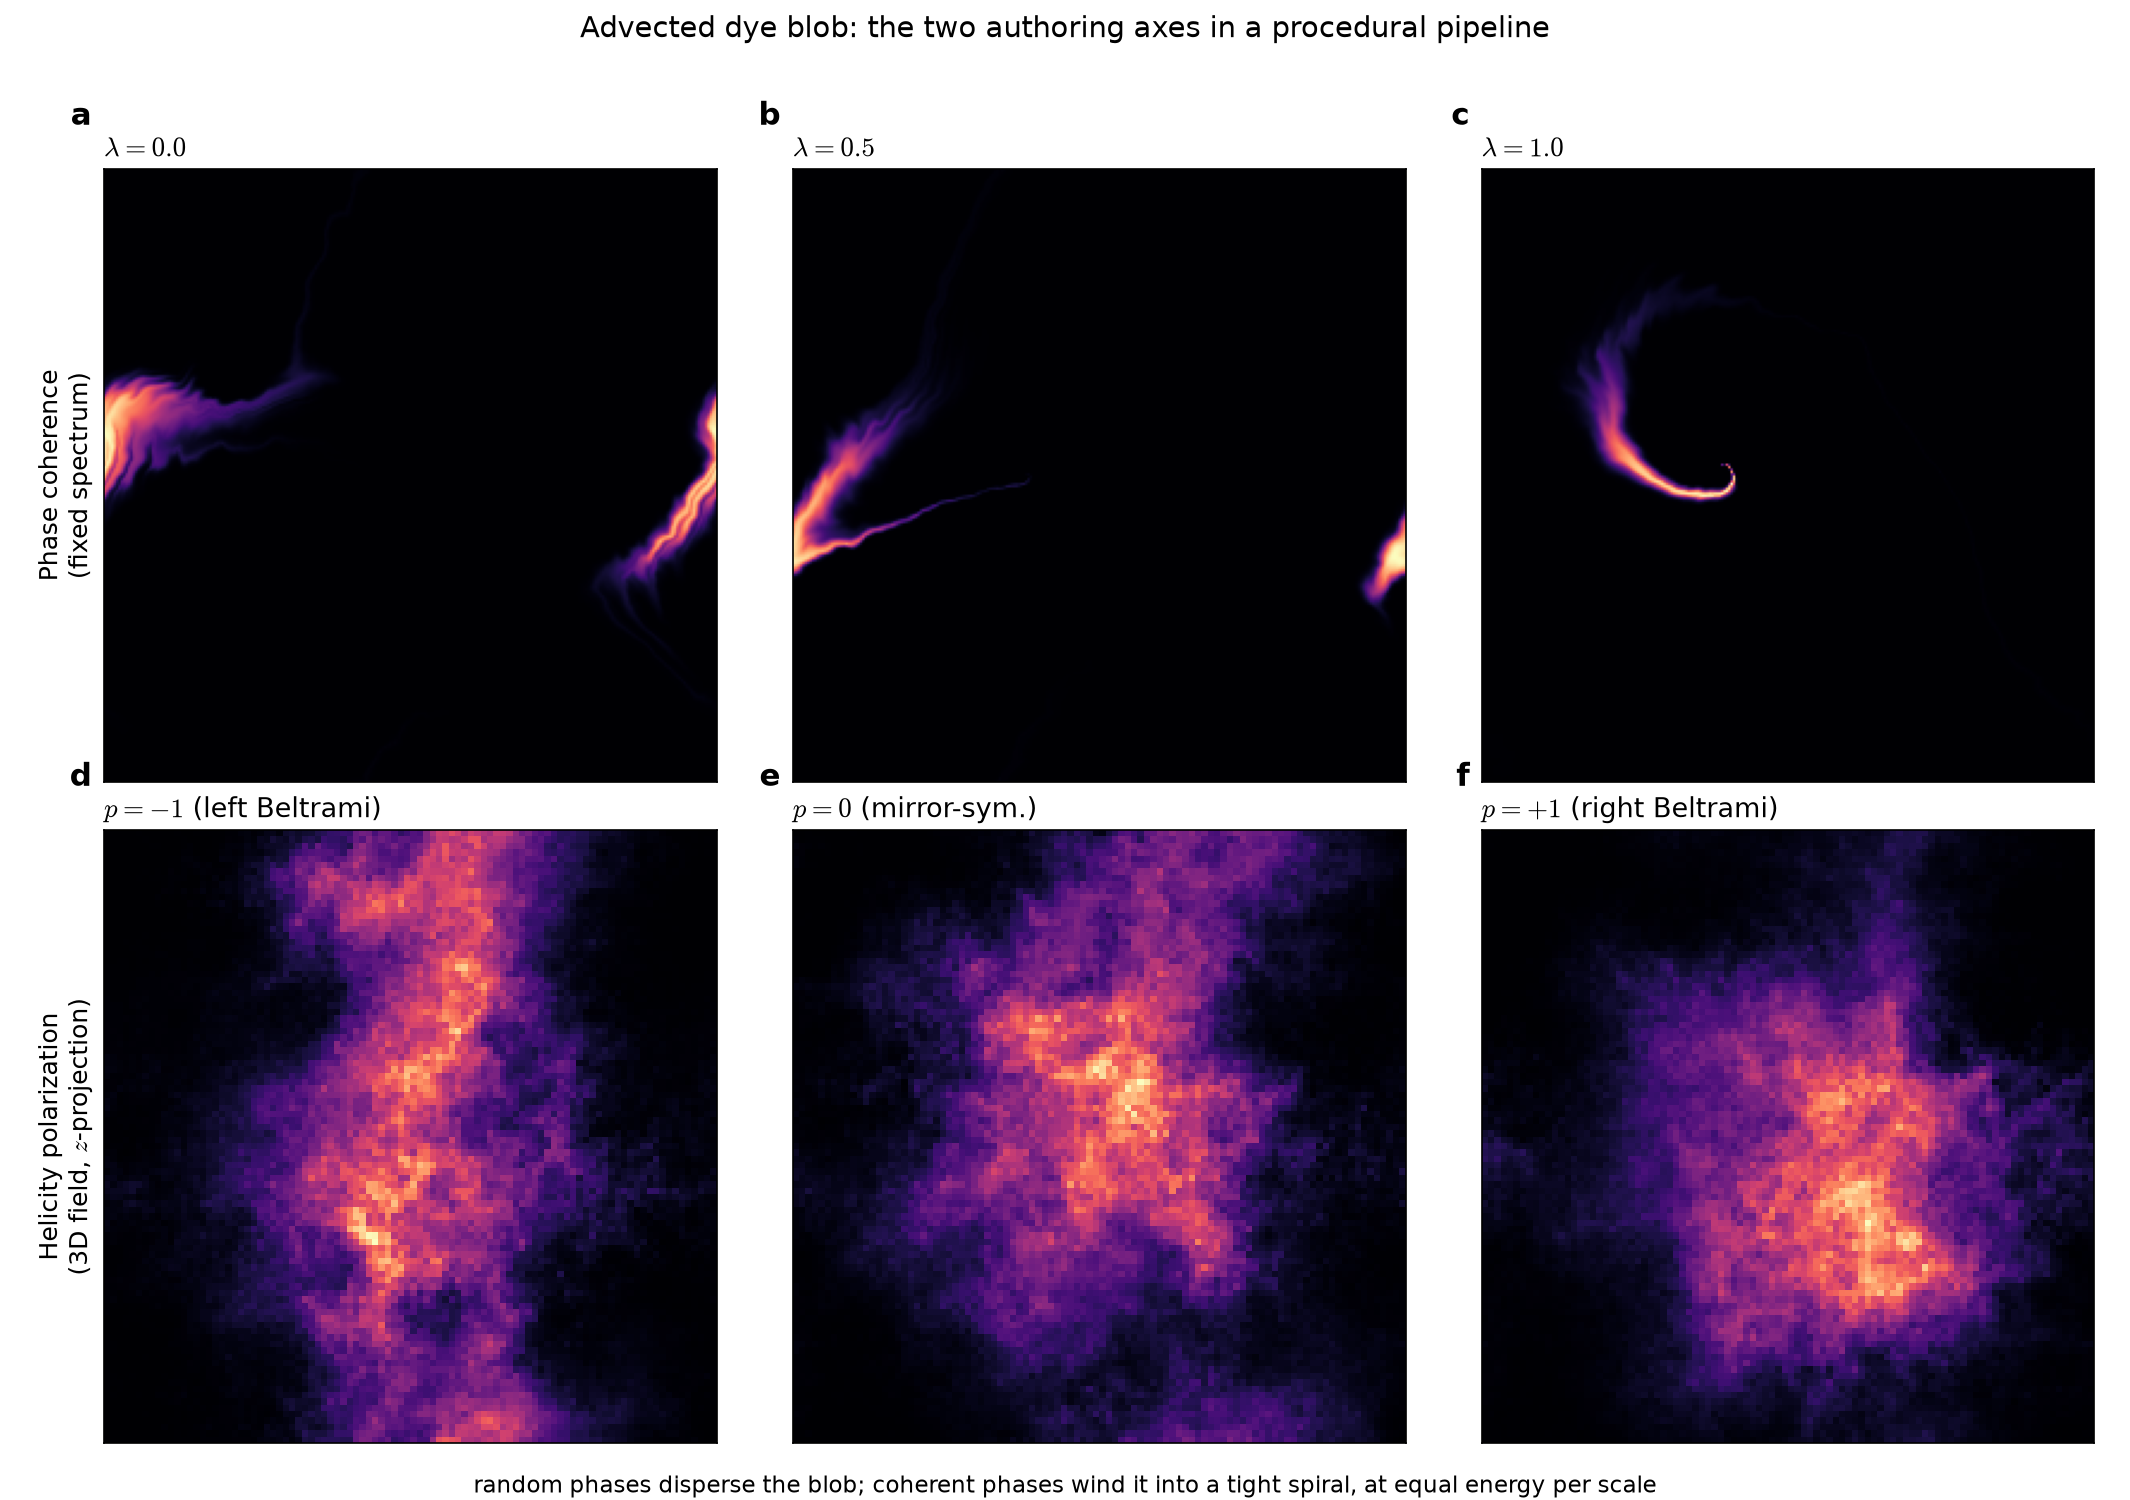
\includegraphics[width=\linewidth]{figures/advection.png}
  \caption{Both axes drive the standard procedural pipeline. A compact dye blob
    is transported by semi-Lagrangian advection through the steady field;
    brightness is the advected dye. \textbf{Top:} the phase-coherence knob---at
    $\lambda=0$ the blob disperses into scattered streaks, while $\lambda=1$ winds it
    into a single tight coherent spiral. \textbf{Bottom:} the helicity
    polarization $p$. The transport needs no pressure projection, the field being
    divergence-free by construction.}
  \label{fig:advection}
\end{figure}

\paragraph{Conclusion.} Building divergence-free fields on the helical basis gives the artist
three independent dials---the spectral slope, the chirality (helicity), and the degree of
organization at fixed spectrum (phase coherence)---the latter two otherwise inaccessible to
curl-noise, all continuously variable and all keeping divergence-freeness exact. The same
potential-ramp mechanism handles solid obstacles with a measured free-slip, no-penetration
guarantee and no solver (\S\ref{sec:obstacles}). The constructions are elementary and
reproducible.

\paragraph{Acknowledgements.} I am grateful to Christopher Batty for generously engaging with
this work and for valuable feedback and encouragement on an earlier draft.

\paragraph{Code and data availability.} All code and data are available at
\url{https://github.com/rifmj/helical-fields}
(DOI: \href{https://doi.org/10.5281/zenodo.21246333}{10.5281/zenodo.21246333}). Every number
reported in this paper is regenerated by a pinned-seed script via \texttt{make reproduce},
and every figure is regenerated from source via \texttt{make figures}.

\appendix

\FloatBarrier
\section{Proof of Proposition~\ref{prop:pres} and implementation notes}
\label{app:hermitian}

\begin{proof}[Proof of Proposition~\ref{prop:pres}]
With $\khat(-\bk)=-\khat(\bk)$ and the stated frame convention,
$\he_+(-\bk)=\tfrac{1}{\sqrt2}(\ehat_1(-\bk)+i\,\ehat_2(-\bk))
=\tfrac{1}{\sqrt2}(\ehat_1(\bk)-i\,\ehat_2(\bk))=\overline{\he_+(\bk)}=\he_-(\bk)$, which
is~\eqref{eq:parity}. Write
$\hat\bu(\bk)=a_+\he_+(\bk)+a_-\he_-(\bk)$. Then
$\overline{\hat\bu(\bk)}=\overline{a_+}\,\overline{\he_+(\bk)}+\overline{a_-}\,
\overline{\he_-(\bk)} =\overline{a_+}\,\he_-(\bk)+\overline{a_-}\,\he_+(\bk)$.
Expanding $\hat\bu(-\bk)=b_+\he_+(-\bk)+b_-\he_-(-\bk)=b_+\he_-(\bk)+b_-\he_+(\bk)$
and matching to $\overline{\hat\bu(\bk)}$ gives $b_+=\overline{a_+}$, $b_-=\overline{a_-}$.
Hence $|a_+(-\bk)|=|a_+(\bk)|$ and likewise for $a_-$; substituting into~\eqref{eq:helicity}
and pairing $\pm\bk$ gives the stated half-space sum. The symmetrization conjugates phases; it
moves no energy between the $\pm$ channels.
\end{proof}

\begin{remark}[convention]
The conclusion depends on the antipodal frame choice $\ehat_2(-\bk)=-\ehat_2(\bk)$; the
opposite choice $\ehat_2(-\bk)=+\ehat_2(\bk)$ would instead swap the $\pm$ channels between
$\bk$ and $-\bk$. In practice one need not track the frame at $-\bk$ at all: assembling
$\hat\bu(\bk)$ on a spectral half-space and setting $\hat\bu(-\bk)=\overline{\hat\bu(\bk)}$
directly realizes the preserving convention.
\end{remark}

\begin{remark}[Nyquist plane]
On an $N^d$ grid the Nyquist frequencies ($k_i=-N/2$ on some axis) are self-conjugate under
the discrete Fourier modular arithmetic and have no distinct $-\bk$ partner; na\"ive
mirror-conjugation there leaks divergence. The fix is to zero the Nyquist plane. With the
cutoff $k_c\ll N/2$ of~\eqref{eq:env} these modes carry negligible energy, but a robust
implementation zeroes them explicitly.
\end{remark}

\begin{thebibliography}{99}
\itemsep2pt

\bibitem{bridson2007}
R.~Bridson, J.~Hourihan, and M.~Nordenstam.
\newblock Curl-noise for procedural fluid flow.
\newblock {\em ACM Transactions on Graphics} 26(3) (SIGGRAPH 2007), Article~46.

\bibitem{perlin1985}
K.~Perlin.
\newblock An image synthesizer.
\newblock {\em Computer Graphics} (SIGGRAPH '85) 19(3):287--296, 1985.

\bibitem{stam1993}
J.~Stam and E.~Fiume.
\newblock Turbulent wind fields for gaseous phenomena.
\newblock In {\em Proc.\ SIGGRAPH '93}, pages 369--376, 1993.

\bibitem{kim2008}
T.~Kim, N.~Th\"urey, D.~James, and M.~Gross.
\newblock Wavelet turbulence for fluid simulation.
\newblock {\em ACM Transactions on Graphics} 27(3) (SIGGRAPH 2008), Article~50.

\bibitem{waleffe1992}
F.~Waleffe.
\newblock The nature of triad interactions in homogeneous turbulence.
\newblock {\em Physics of Fluids A} 4(2):350--363, 1992.

\bibitem{constantin1988}
P.~Constantin and A.~Majda.
\newblock The Beltrami spectrum for incompressible fluid flows.
\newblock {\em Communications in Mathematical Physics} 115(3):435--456, 1988.

\bibitem{herring1974}
J.~R.~Herring.
\newblock Approach of axisymmetric turbulence to isotropy.
\newblock {\em Physics of Fluids} 17(5):859--872, 1974.

\bibitem{moffatt1969}
H.~K.~Moffatt.
\newblock The degree of knottedness of tangled vortex lines.
\newblock {\em Journal of Fluid Mechanics} 35(1):117--129, 1969.

\bibitem{dombre1986}
T.~Dombre, U.~Frisch, J.~M.~Greene, M.~H\'enon, A.~Mehr, and A.~M.~Soward.
\newblock Chaotic streamlines in the ABC flows.
\newblock {\em Journal of Fluid Mechanics} 167:353--391, 1986.

\bibitem{coles2000}
P.~Coles and L.-Y.~Chiang.
\newblock Characterizing the nonlinear growth of large-scale structure in the Universe.
\newblock {\em Nature} 406:376--378, 2000.

\bibitem{chern2016}
A.~Chern, F.~Kn\"oppel, U.~Pinkall, P.~Schr\"oder, and S.~Wei{\ss}mann.
\newblock Schr\"odinger's smoke.
\newblock {\em ACM Transactions on Graphics} 35(4), SIGGRAPH 2016.
\newblock \href{https://doi.org/10.1145/2897824.2925868}{doi:10.1145/2897824.2925868}.

\bibitem{ishida2022}
S.~Ishida, C.~Wojtan, and A.~Chern.
\newblock Hidden degrees of freedom in implicit vortex filaments.
\newblock {\em ACM Transactions on Graphics} 41(6), SIGGRAPH Asia 2022.
\newblock \href{https://doi.org/10.1145/3550454.3555459}{doi:10.1145/3550454.3555459}.

\bibitem{chang2022}
J.~Chang, R.~Partono, V.~C.~Azevedo, and C.~Batty.
\newblock Curl-Flow: boundary-respecting pointwise incompressible velocity
interpolation for grid-based fluids.
\newblock {\em ACM Transactions on Graphics} 41(6), SIGGRAPH Asia 2022.
\newblock \href{https://doi.org/10.1145/3550454.3555498}{doi:10.1145/3550454.3555498}.

\bibitem{ding2023}
X.~Ding and C.~Batty.
\newblock Differentiable curl-noise.
\newblock {\em Proceedings of the ACM on Computer Graphics and Interactive
Techniques} 6(1), 2023.
\newblock \href{https://doi.org/10.1145/3585511}{doi:10.1145/3585511}.

\bibitem{lagae2010}
A.~Lagae, S.~Lef\`ebvre, R.~Cook, T.~DeRose, G.~Drettakis, D.~S.~Ebert,
J.~P.~Lewis, K.~Perlin, and M.~Zwicker.
\newblock A survey of procedural noise functions.
\newblock {\em Computer Graphics Forum} 29(8):2579--2600, 2010.
\newblock \href{https://doi.org/10.1111/j.1467-8659.2010.01827.x}{doi:10.1111/j.1467-8659.2010.01827.x}.

\bibitem{galerne2012}
B.~Galerne, A.~Lagae, S.~Lef\`ebvre, and G.~Drettakis.
\newblock Gabor noise by example.
\newblock {\em ACM Transactions on Graphics} 31(4), SIGGRAPH 2012.
\newblock \href{https://doi.org/10.1145/2185520.2185569}{doi:10.1145/2185520.2185569}.

\bibitem{sato2021}
S.~Sato, Y.~Dobashi, and T.~Kim.
\newblock Stream-guided smoke simulations.
\newblock {\em ACM Transactions on Graphics} 40(4), SIGGRAPH 2021.
\newblock \href{https://doi.org/10.1145/3450626.3459846}{doi:10.1145/3450626.3459846}.

\bibitem{wang2024}
X.~Wang, Y.~Xu, S.~Liu, B.~Ren, J.~Bender, et al.
\newblock Physics-based fluid simulation in computer graphics: survey, research
trends, and challenges.
\newblock {\em Computational Visual Media} 10(5):803--858, 2024.
\newblock \href{https://doi.org/10.1007/s41095-023-0368-y}{doi:10.1007/s41095-023-0368-y}.

\end{thebibliography}

\end{document}
